\chapter{Missing epidemiologic parameter data: transport injuries}
\label{applications-double_dismod}

For whatever reason, data are often not available for one or more
epidemiological parameters.  In the GBD 2010 study, this is
problematic when the missing parameter is needed for the calculation
of disease burden.  Injuries provide an excellent example of missing
epidemiologic parameter data as incidence is often only reported.

In the GBD 2010 Study, injuries are defined as conditions codable to
the ICD-9 and ICD-10 injuries chapter.  Transport injuries includes
all road injuries for pedestrian, bicyclist, motorized two-wheeler
rider, occupant in a motorized vehicle with 3 or more wheels, other
road-transport injury and unintentional other transport injury.

Data only include cases warranting hospital care and cases warranting
treatment by health care professional but not hospitalization (other
health care).  As seen in Figure \ref{fig:app-injury traffic data},
only incidence and cause-specific mortality were available from verbal
autopsy, surveillance systems, surveys, census and police reports.
Cause-specific mortality assumes that anyone who died with the
condition died of the condition.

    \begin{figure}[h]
        \begin{center}
            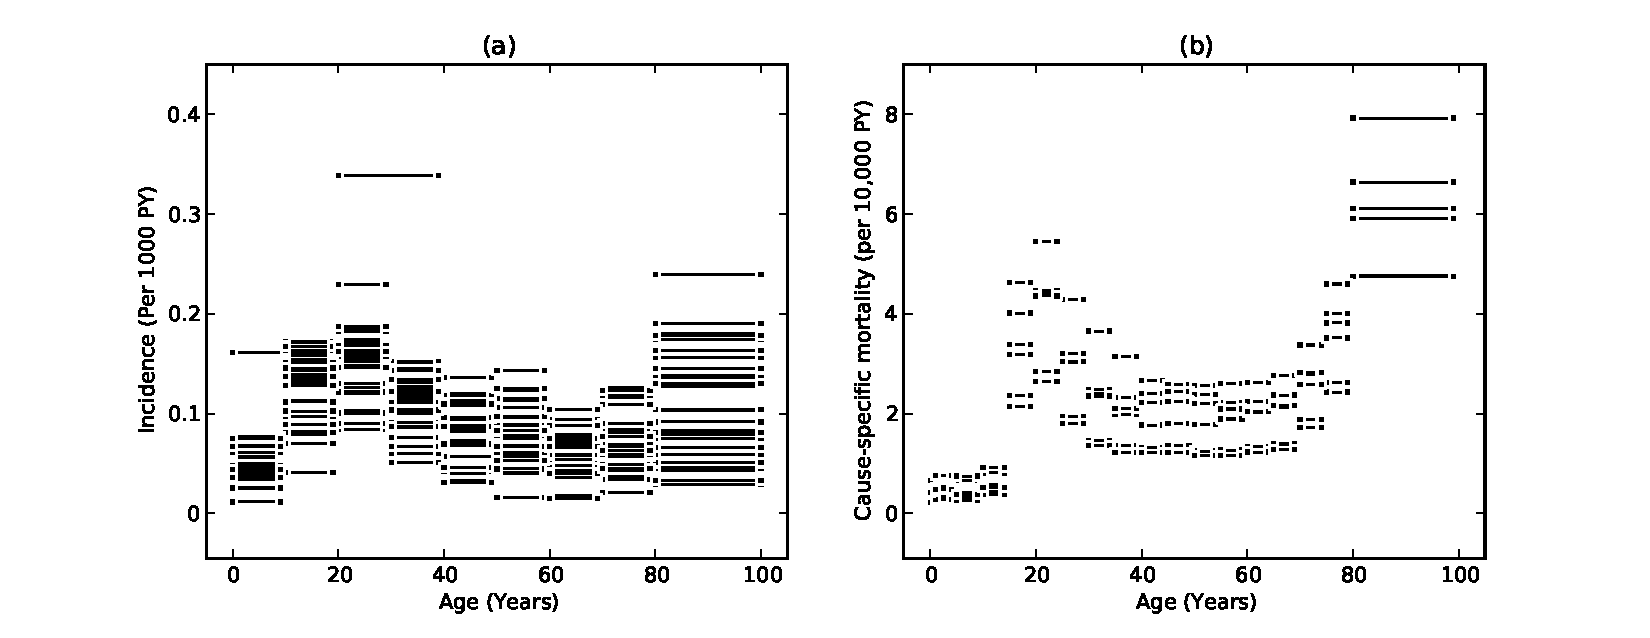
\includegraphics[width=\textwidth]{injury-traffic_data.pdf}
            \caption{Incidence (panel (a)) and cause-specific
              mortality (panel (b)) data for transport injuries for
              males in the region of North America, High Income.}
            \label{fig:app-injury traffic data}
        \end{center}
    \end{figure}

To estimate prevalence, both the cause-specific mortality and the
incidence data are used in a compartmental model to estimate the
age-specific burden of transport injuries, as shown in Figure
\ref{fig:app-injury traffic fit}.  By fitting all of the epidemiologic
parameters together, the compartmental model can estimate prevalence
without prevalence data.

    \begin{figure}[h]
        \begin{center}
            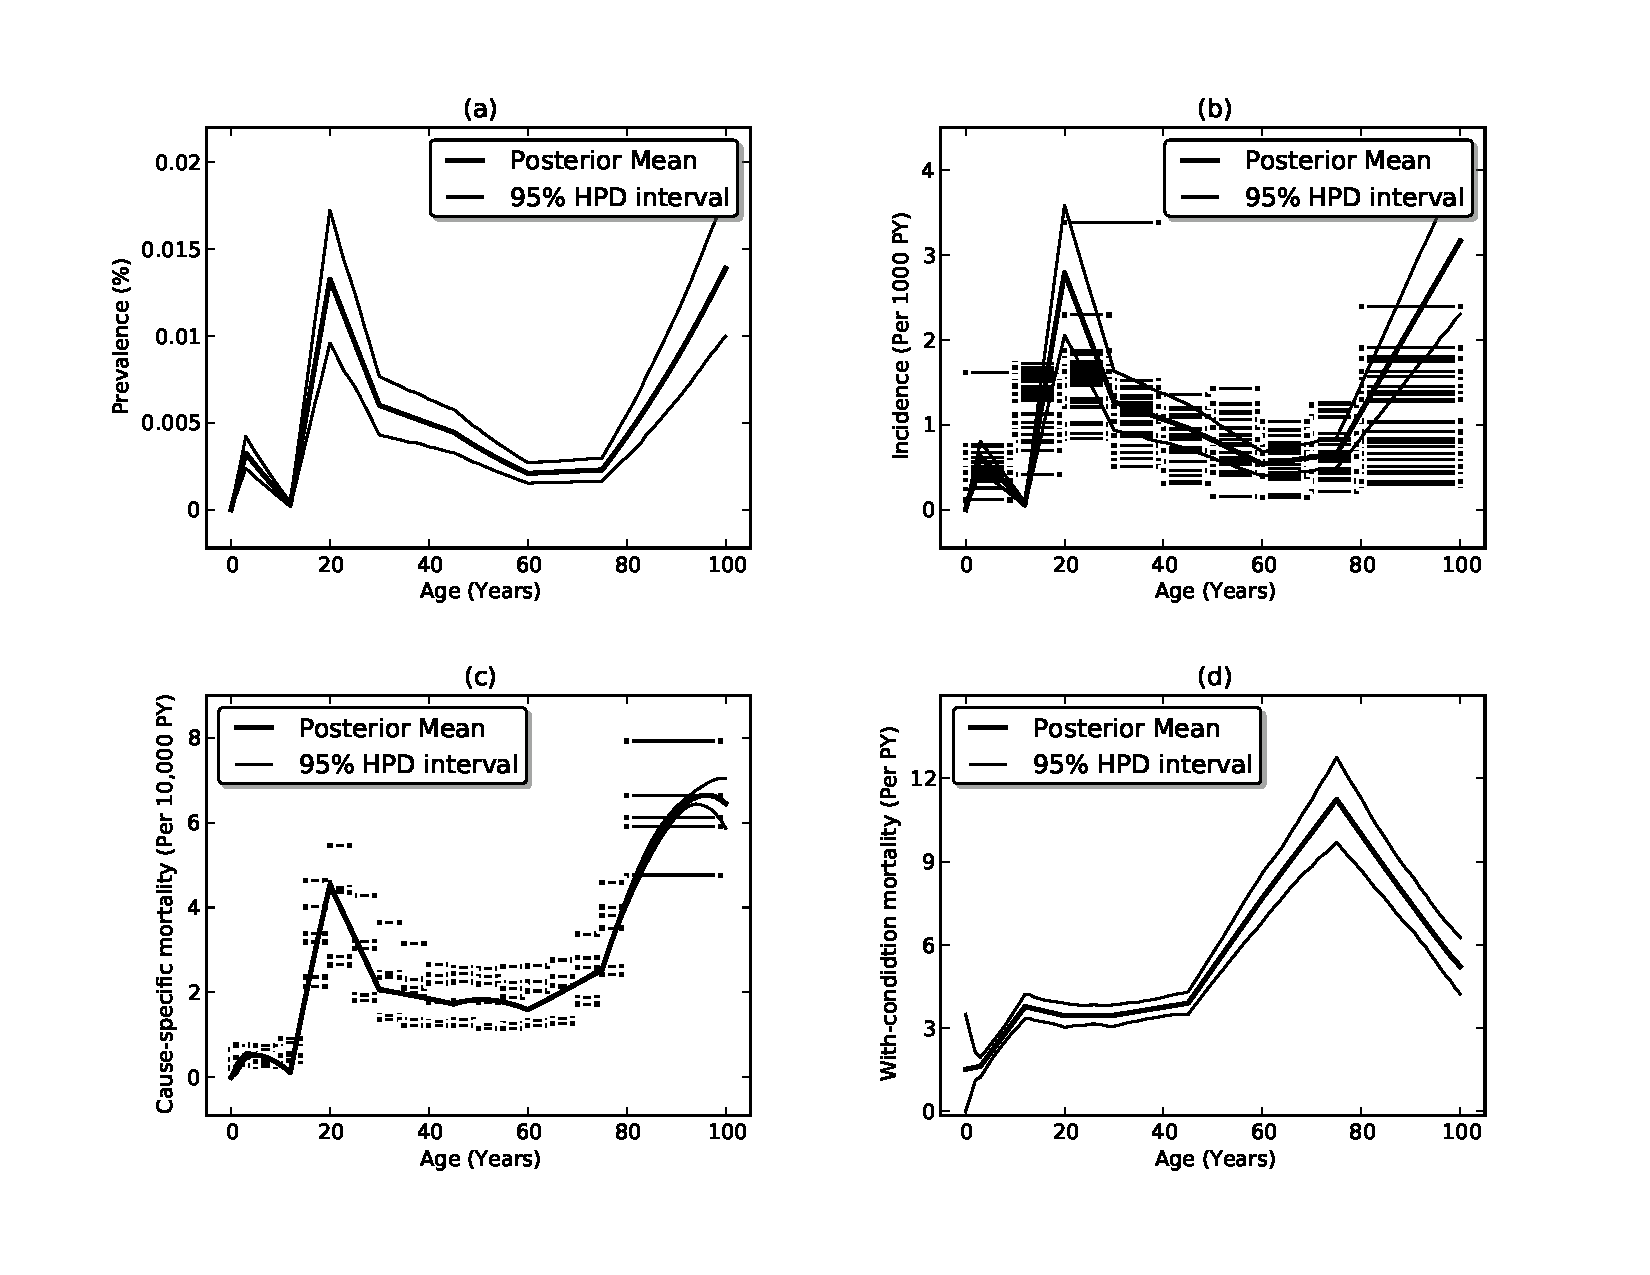
\includegraphics[width=\textwidth]{injuries-traffic_con_fit.pdf}
            \caption{A compartmental model estimates the prevalence
              (panel (a)), incidence (panel (b)), cause-specific
              mortality (panel (c)) and with-condition mortality
              (panel (d)) for males in the United States of America in
              2005.}
            \label{fig:app-injury traffic fit}
        \end{center}
    \end{figure}

For most conditions, this is all that is necessary to calculate
disease burden.  However, transport injuries have a wide range of
outcomes, ranging from minor scratches to severe brain trauma to
death.  Given some cases suffer acute injury while others sustain
chronic conditions, the burden of the disease and the mortality hazard
differ by outcome.  Thus the compartmental model is not appropriate
for traffic injuries since it violates the model assumption of a
constant mortality hazard.  To address this disparity in mortality
risk, transport injuries can be divided into short term and long term
outcomes.  This method is also necessary for other injuries and
diseases such as heart attack and stroke.

Dividing incidence into short and long term outcomes avoids violating
the assumption of a constant mortality hazard.  Once long term traffic
injury incidence is extracted, it is further subdivided into the
nature of the injury, such as fractures, burns, amputations or
traumatic brain injury.  Systematic review only yields traumatic brain
injury incidence.  Again, the compartmental model simultaneously fits
all epidemiologic parameters to estimate traumatic brain injury
prevalence, as see in Figure \ref{fig:app-injury brain fit}.

    \begin{figure}[h]
        \begin{center}
            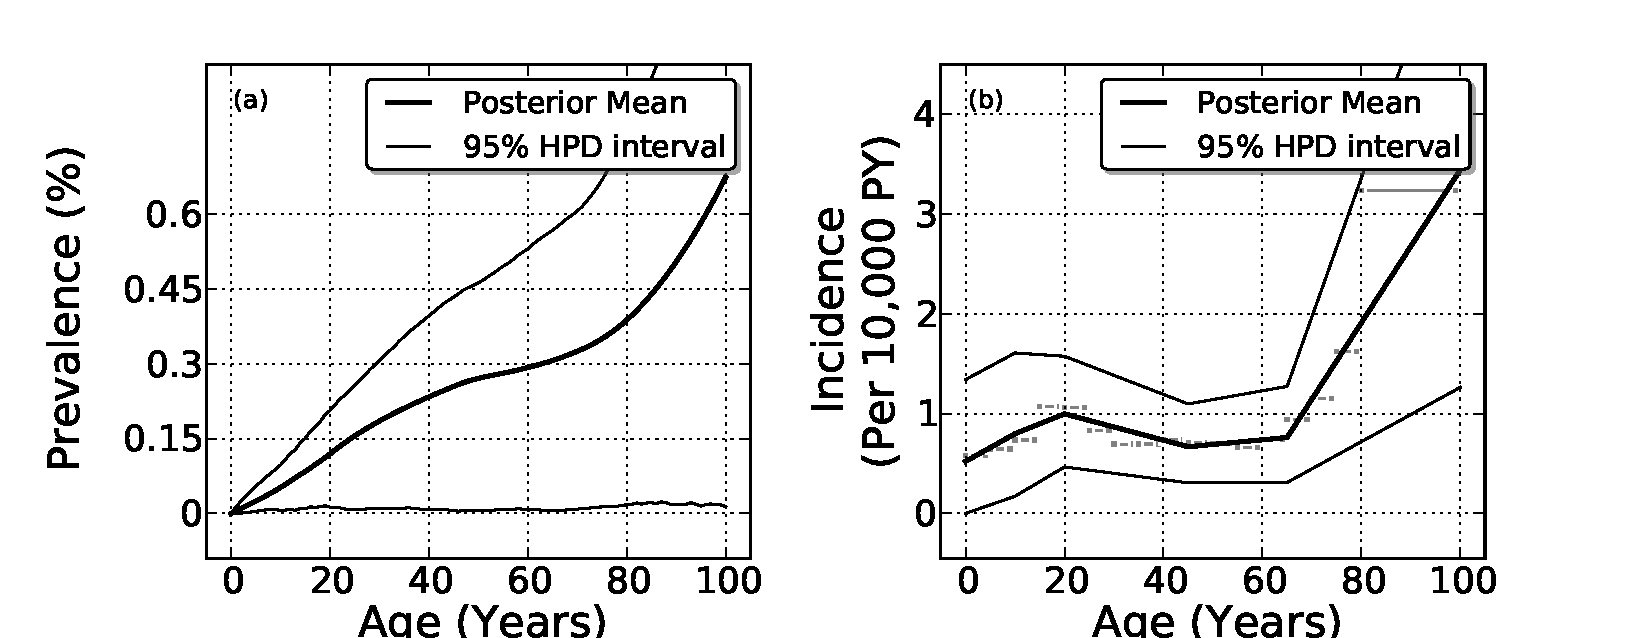
\includegraphics[width=\textwidth]{injuries-con_fit_p.pdf}
            \caption{Prevalence (panel (a)) and incidence (panel (b))
              estimates for males in the United States of America in
              2005 with moderate to severe traumatic brain injury
              caused by traffic injuries.}
            \label{fig:app-injury brain fit}
        \end{center}
    \end{figure}



